\documentclass[11pt,a4paper]{article}
\usepackage[margin=23mm,headheight=15pt]{geometry}
\usepackage{fontspec}
\setmainfont{Times New Roman}
\setsansfont{Arial}
\usepackage{amsmath,amssymb,graphicx,booktabs,array,tabularx,longtable,caption,xcolor,fancyhdr,enumitem,placeins}
\usepackage[numbers,sort&compress]{natbib}
\usepackage[colorlinks=true,linkcolor=teal!55!black,citecolor=teal!55!black,urlcolor=teal!55!black]{hyperref}
\definecolor{navy}{HTML}{193447}
\definecolor{pale}{HTML}{EDF4F5}
\usepackage{titlesec}
\titleformat{\section}{\large\sffamily\bfseries\color{navy}}{}{0em}{}
\setlength{\parindent}{0pt}
\setlength{\parskip}{6pt}
\raggedbottom
\setlength{\emergencystretch}{3em}
\widowpenalty=10000\clubpenalty=10000
\renewcommand{\topfraction}{.95}\renewcommand{\bottomfraction}{.85}\renewcommand{\textfraction}{.05}\renewcommand{\floatpagefraction}{.75}
\renewcommand{\arraystretch}{1.16}
\captionsetup{font=small,labelfont=bf,justification=raggedright,singlelinecheck=false}
\pagestyle{fancy}\fancyhf{}\fancyhead[L]{\small\sffamily EVIDENCE TO EXPERIMENT}\fancyhead[R]{\small\sffamily 17 November 2026}\fancyfoot[C]{\thepage}
\renewcommand{\headrulewidth}{0.3pt}
\graphicspath{{figures/}}
\newcounter{boxnum}
\newcommand{\boxlabel}{Box}
\usepackage{xeCJK}
\setCJKmainfont{SimSun}[BoldFont=SimHei,ItalicFont=KaiTi]
\setCJKsansfont{Microsoft YaHei}
\renewcommand{\figurename}{图}\renewcommand{\tablename}{表}\renewcommand{\refname}{参考文献}\renewcommand{\boxlabel}{框}
\begin{document}
{\small\sffamily\color{navy} 补充证据图谱}\par\medskip
{\LARGE\bfseries\raggedright 证据地图与实验选择规则\par}\bigskip
{\normalsize JiaHao Wu、曾龙（Long Zeng）\par}
{\small 清华大学深圳国际研究生院，中国深圳\par}\medskip
\hypersetup{pdfauthor={JiaHao Wu; Long Zeng}}
{\small 通讯作者：曾龙（Long Zeng），\href{mailto:zenglong@sz.tsinghua.edu.cn}{zenglong@sz.tsinghua.edu.cn}\par}\medskip
29个条目分别记录已发表观察、本文综合推断和拟议测试；每项给出文献及原文图、实验或节定位。八张决策卡说明对照与计算边界。覆盖以人类上肢适应为中心，2026年已评审预印本及计算贡献均单独标示；完整双语条目另以JSON提供。
\begin{table}[!htbp]\small\caption{证据支持不同解释层级；编号对应详细图谱。}\label{tab:synthesis}
\begin{tabularx}{\textwidth}{>{\raggedright\arraybackslash}X>{\raggedright\arraybackslash}X>{\raggedright\arraybackslash}X}\toprule
\textbf{证据} & \textbf{已支持推断} & \textbf{整合预测}\\\midrule
迁移（E01--E03、E08） & 动力学知识影响多个输出。 & 交叉训练/测试情境测量跨输出迁移。\\[5pt]
分离（E04--E07、E11） & 耦合依赖暴露与时序。 & 匹配延迟，配对完整纠错与学习波形。\\[5pt]
归因（E13--E16、E19） & 来源与情境影响特定学习/读出成分。 & 交叉来源与持续性，独立校准感知。\\[5pt]
感觉特异性（E12、E17--E18） & 不同感觉输入可产生不同学习后果。 & 同时检验不同输入动态及向两个控制输出的迁移。\\[5pt]
\bottomrule\end{tabularx}\end{table}
\section{证据层级的阅读方式}
观察结果：实验实际测得什么。支持推断：原实验对照约束到的机制层级。残余解释：能产生该观察的具体竞争解释。拟议测试：本文提出的下一对比及其解释价值。保留竞争解释，同时保留原研究已确立的结果。
\clearpage\section{E01 | Shared Internal Models for Feedforward and Feedback Control}
{\small\sffamily\color{navy} 迁移}\par
\textbf{来源} \cite{wagner2008}; Results: responses to unexpected perturbations after force-field learning; model comparisons\par
\textbf{研究类型/状态} 已发表原始研究\par
\textbf{操纵与比较} 训练力场中的到达运动，再在运动中施加非预期扰动。\par
\textbf{测量指标} 不同已学习动力学下的纠错时程与运动轨迹。\par
\textbf{观察结果} 在线纠错利用了力场训练中获得的知识。\par
\textbf{支持的推断} 学到的动力学同时影响预先准备的运动与在线纠错。\par
\textbf{残余解释} 共享动力学估计和经过训练的循环策略均可将已有知识用于纠错。\par
\textbf{可区分预测/拟议追加测量} 匹配基线轨迹；固定训练后的参数，预测未训练扰动方向和时点的响应。\par
\bigskip\hrule\medskip\section{E02 | Feedforward and Feedback Control Share an Internal Model of the Arm's Dynamics}
{\small\sffamily\color{navy} 迁移}\par
\textbf{来源} \cite{maeda2018}; Figures 3, 6 and 7; shoulder-fixation and no-fixation control\par
\textbf{研究类型/状态} 已发表原始研究\par
\textbf{操纵与比较} 自主肘关节到达训练时固定肩关节；机械扰动测试时释放肩关节。\par
\textbf{测量指标} 到达运动肩部肌电及扰动后50--100 ms长潜伏期响应；扰动前肌电与肘部肌肉对照。\par
\textbf{观察结果} 训练中的肩部激活下降迁移至肩部长潜伏期响应。\par
\textbf{支持的推断} 迁移涉及快速反馈通路，并有基线肌电对照。\par
\textbf{残余解释} 共享存储、耦合更新与共同的任务依赖读出均可实现该现象。\par
\textbf{可区分预测/拟议追加测量} 交叉训练与测试情境，同时测量扰动前肌电、短潜伏期及长潜伏期响应。\par
\clearpage\section{E03 | Learning New Feedforward Motor Commands Based on Feedback Responses}
{\small\sffamily\color{navy} 迁移}\par
\textbf{来源} \cite{maeda2020}; Figures 3--4; perturbation training and transfer-to-reaching probes\par
\textbf{研究类型/状态} 已发表原始研究\par
\textbf{操纵与比较} 固定肩关节、减少主动介入，训练机械扰动响应，再探测自主到达运动。\par
\textbf{测量指标} 训练中的肩部长潜伏期响应与到达探针中的预期性肩部肌电。\par
\textbf{观察结果} 反馈训练改变了之后的自主运动指令。\par
\textbf{支持的推断} 迁移可从反馈训练指向自主控制，与反方向证据相互补充。\par
\textbf{残余解释} 双向迁移可由共同表征或不同表征间的信息传递产生。\par
\textbf{可区分预测/拟议追加测量} 在两个方向使用匹配延迟测量迁移，并在相同探针情境下比较学习与保持。\par
\bigskip\hrule\medskip\section{E04 | Structural learning in feedforward and feedback control}
{\small\sffamily\color{navy} 分离}\par
\textbf{来源} \cite{yousif2012}; Experiments 1--3; Figures 4--6, especially Figure 6\par
\textbf{研究类型/状态} 已发表原始研究\par
\textbf{操纵与比较} 匹配力场、零力场和通道试次数量，改变位置相关力场暴露的时间一致性。\par
\textbf{测量指标} 前馈适应及目标---通道错位反馈中，通道力的位置与速度成分。\par
\textbf{观察结果} 一致暴露改变两个控制域；不一致暴露改变反馈结构，未产生相应的前馈结构变化。\par
\textbf{支持的推断} 误差的时间统计影响所测控制输出之间的耦合。\par
\textbf{残余解释} 不同更新规则、时间尺度或情境依赖表达均可产生该分离。\par
\textbf{可区分预测/拟议追加测量} 增加共同测试情境下的多延迟探针；匹配读出后仍持续的差异支持学习或保持差异。\par
\clearpage\section{E05 | Learning feedback and feedforward control in a mirror-reversed visual environment}
{\small\sffamily\color{navy} 分离}\par
\textbf{来源} \cite{kasuga2015}; Figures 3--5; endpoint, online and no-mirror control groups\par
\textbf{研究类型/状态} 已发表原始研究\par
\textbf{操纵与比较} 在镜像反转条件下，使用终点视觉反馈或连续视觉反馈训练。\par
\textbf{测量指标} 初始运动方向与光标跳变引起的力响应；主要分析窗为251--350 ms。\par
\textbf{观察结果} 终点反馈更有利于前馈表现；在线反馈暴露使不适当反馈响应的衰减更明显。\par
\textbf{支持的推断} 在线动作后果的暴露影响新反馈策略的获得。\par
\textbf{残余解释} 镜像反转要求策略重映射，其训练时长与感觉暴露不同于力场适应。\par
\textbf{可区分预测/拟议追加测量} 匹配感觉暴露与稳定后的基线表现，再跨训练时长比较完整响应波形。\par
\bigskip\hrule\medskip\section{E06 | The Neural Feedback Response to Error As a Teaching Signal for the Motor Learning System}
{\small\sffamily\color{navy} 教学信号}\par
\textbf{来源} \cite{albert2016}; Figures 1, 5--6; 2016 correction concerns Figure 2A Error 2 displacement traces\par
\textbf{研究类型/状态} 已发表原始研究\par
\textbf{操纵与比较} 在基线与误差后通道试次之间插入一至两个旋转力场试次。\par
\textbf{测量指标} 跨肌肉比较扰动减基线肌电、误差后减基线肌电。\par
\textbf{观察结果} 学习相关肌电近似于缩放后、提前约125 ms的纠错响应。\par
\textbf{支持的推断} 该力场范式的肌肉模式支持与反馈有关的教学信号。\par
\textbf{残余解释} 共同上游误差信号也可使两类响应相关；时间复制假说需额外时序操纵。\par
\textbf{可区分预测/拟议追加测量} 改变扰动起始时点并反转晚期误差，配对测量纠错与下一试次力/肌电，同时预测时序与幅值。\par
\clearpage\section{E07 | Tonic feedback motor commands predict visuomotor learning}
{\small\sffamily\color{navy} 教学信号}\par
\textbf{来源} \cite{makino2026}; Experiments 1--3; Figures 1--4; reviewed preprint v1, 29 June 2026\par
\textbf{研究类型/状态} 已评审预印本第1版\par
\textbf{操纵与比较} 在力通道内操纵光标位移的起始时点、幅度和时间模式。\par
\textbf{测量指标} 扣除基线的纠错力与下一试次学习力，包括末端保持期。\par
\textbf{观察结果} 学习响应的起始保持与运动开始对齐；持续保持响应可预测不同视觉误差模式下的学习幅度。\par
\textbf{支持的推断} 视觉误差时序实验约束了普适固定时间平移复制解释。\par
\textbf{残余解释} 持续力可能反映整合后的教学变量；其因果中介作用及向力场误差的推广有待检验。\par
\textbf{可区分预测/拟议追加测量} 匹配视觉与机械扰动时序，比较预先指定的复制模型与时间整合模型对留出时序的预测。\par
\bigskip\hrule\medskip\section{E08 | Rapid Feedback Responses Correlate with Reach Adaptation and Properties of Novel Upper Limb Loads}
{\small\sffamily\color{navy} 迁移}\par
\textbf{来源} \cite{cluff2013}; Results: load magnitude/direction and rapid-feedback adaptation\par
\textbf{研究类型/状态} 已发表原始研究\par
\textbf{操纵与比较} 对不同大小和方向的新上肢负载进行到达适应训练。\par
\textbf{测量指标} 在控制背景激活的探针目标处测量到达适应与扰动诱发的快速肌肉响应。\par
\textbf{观察结果} 反馈变化与到达适应及已学习负载的属性相关。\par
\textbf{支持的推断} 反馈调节包含负载特异信息。\par
\textbf{残余解释} 背景激活对照约束自动增益缩放；共同估计与联合训练输出仍是竞争实现。\par
\textbf{可区分预测/拟议追加测量} 在匹配背景激活下测量增益缩放，并测试未见过的负载---目标组合。\par
\clearpage\section{E09 | Adaptation to Stable and Unstable Dynamics Achieved By Combined Impedance Control and Inverse Dynamics Model}
{\small\sffamily\color{navy} 力学}\par
\textbf{来源} \cite{franklin2003}; Stable velocity field versus unstable divergent field; Figures 5--10\par
\textbf{研究类型/状态} 已发表原始研究\par
\textbf{操纵与比较} 比较稳定速度相关动力学与不稳定发散动力学下的适应。\par
\textbf{测量指标} 学习过程中的轨迹、力/力矩与肌肉激活。\par
\textbf{观察结果} 适应成功伴随补偿指令与共激活变化，其组合取决于环境稳定性。\par
\textbf{支持的推断} 身体力学变化可参与产生相似的轨迹精度改善。\par
\textbf{残余解释} 肌电共激活是刚度的间接指标；神经反馈与内在力学共同影响抗扰。\par
\textbf{可区分预测/拟议追加测量} 增加小幅多方向机械探针、背景肌电与按潜伏期分解的力响应，独立估计阻抗。\par
\bigskip\hrule\medskip\section{E10 | Visuomotor feedback tuning in the absence of visual error information}
{\small\sffamily\color{navy} 分离}\par
\textbf{来源} \cite{franklin2023}; Results: visual-error availability, feedback gains and co-contraction\par
\textbf{研究类型/状态} 已发表原始研究\par
\textbf{操纵与比较} 改变力场突然或渐进引入方式，以及视觉轨迹误差的可用性。\par
\textbf{测量指标} 适应、视运动反馈增益与共收缩。\par
\textbf{观察结果} 移除视觉误差降低反馈增益，同时保留与学习有关的调节模式。\par
\textbf{支持的推断} 所测视觉增益同时依赖感觉条件与训练状态。\par
\textbf{残余解释} 基于不确定性的解释需要独立测量不确定性。\par
\textbf{可区分预测/拟议追加测量} 在学习之外校准视觉可靠性与纠错增益，再预测跨可靠性操纵的迁移。\par
\clearpage\section{E11 | Feedback Adaptation to Unpredictable Force Fields in 250 ms}
{\small\sffamily\color{navy} 时间尺度}\par
\textbf{来源} \cite{crevecoeur2020}; Experiments 1--2; Figures 3--7\par
\textbf{研究类型/状态} 已发表原始研究\par
\textbf{操纵与比较} 随机呈现不可预期的力场，并包含不同力场类型。\par
\textbf{测量指标} 单次到达中的肌电、力与运动晚期运动学。\par
\textbf{观察结果} 反馈在运动开始后约250 ms的时间尺度上表现出对当前力场的调谐。\par
\textbf{支持的推断} 与适应有关的调整可在一次正在进行的运动内发生。\par
\textbf{残余解释} 快速辨识与已有策略之间的选择均可产生相关的试次内变化。\par
\textbf{可区分预测/拟议追加测量} 在匹配试次内纠错后探测下一试次，检验变化是否保持与泛化。\par
\bigskip\hrule\medskip\section{E12 | Learning from Sensory and Reward Prediction Errors during Motor Adaptation}
{\small\sffamily\color{navy} 读出}\par
\textbf{来源} \cite{izawa2011}; Sensory versus reward prediction-error training; sensory remapping and generalization results\par
\textbf{研究类型/状态} 已发表原始研究\par
\textbf{操纵与比较} 比较感觉预测误差驱动训练与奖励驱动学习。\par
\textbf{测量指标} 运动适应、所报告的感觉后果及泛化。\par
\textbf{观察结果} 不同学习途径在运动表现变化之外，产生可区分的感觉重映射。\par
\textbf{支持的推断} 配对感觉读出能够约束学习伴随的内部后果。\par
\textbf{残余解释} 感觉报告依赖任务、估计与报告映射。\par
\textbf{可区分预测/拟议追加测量} 增加报告映射一致的被动与主动定位，并匹配运动表现。\par
\clearpage\section{E13 | Estimating the sources of motor errors for adaptation and generalization}
{\small\sffamily\color{navy} 来源归因}\par
\textbf{来源} \cite{berniker2008}; Model and comparisons with published generalization experiments; Figures 1--5\par
\textbf{研究类型/状态} 计算理论及既有实验比较\par
\textbf{操纵与比较} 建模身体与外部世界动力学的潜在变化，并与已发表实验的迁移结果比较。\par
\textbf{测量指标} 跨工作空间、肢体及物体情境的泛化预测。\par
\textbf{观察结果} 推断出的不同扰动来源产生不同泛化模式。\par
\textbf{支持的推断} 来源推断为结构化泛化提供了计算解释。\par
\textbf{残余解释} 来源估计模型的拟合支持其解释能力；其他潜状态模型可能给出相同预测。\par
\textbf{可区分预测/拟议追加测量} 在匹配物理误差时改变来源线索，并预先指定对未训练肢体或物体的预测。\par
\bigskip\hrule\medskip\section{E14 | Relevance of Error: What Drives Motor Adaptation?}
{\small\sffamily\color{navy} 来源归因}\par
\textbf{来源} \cite{wei2009}; Experiments manipulating error magnitude; relevance model\par
\textbf{研究类型/状态} 已发表原始研究\par
\textbf{操纵与比较} 改变到达适应中的感觉误差幅度。\par
\textbf{测量指标} 随误差大小变化的试次间适应。\par
\textbf{观察结果} 误差敏感性随误差幅度非线性变化，支持误差相关性估计解释。\par
\textbf{支持的推断} 学习增益依赖误差幅度之外的因素。\par
\textbf{残余解释} 饱和编码与信念变化均可产生相关的输入---输出曲线。\par
\textbf{可区分预测/拟议追加测量} 交叉操纵误差大小与独立的来源可信度，同时测量感知误差和学习。\par
\clearpage\section{E15 | External error attribution dampens efferent-based predictions but not proprioceptive changes in hand localization}
{\small\sffamily\color{navy} 来源归因}\par
\textbf{来源} \cite{external2020}; Results: reach aftereffects, passive localization, active-minus-passive localization; hand-view and cursor-jump groups\par
\textbf{研究类型/状态} 已发表原始研究\par
\textbf{操纵与比较} 通过可见光标跳变或直接看到手的位置揭示视运动旋转。\par
\textbf{测量指标} 到达后效、被动定位及主动减被动定位。\par
\textbf{观察结果} 揭示条件下后效减小，被动定位变化保留；手可见组主动减被动估计接近零，其与对照组的直接差异仍有不确定性。\par
\textbf{支持的推断} 运动后效与报告成分呈不同响应模式；手可见对比对传出机制是否消除保留多种解释。\par
\textbf{残余解释} 看到手同时改变感觉信息与归因；主动减被动定位依赖差分假设。\par
\textbf{可区分预测/拟议追加测量} 增加手可见性相同的可信纯线索归因条件，并独立校准定位测量。\par
\bigskip\hrule\medskip\section{E16 | Causal inference, prediction and state estimation in sensorimotor learning}
{\small\sffamily\color{navy} 来源归因}\par
\textbf{来源} \cite{piece2025}; Figure 1 experimental setup; Figure 2 human results; model comparisons\par
\textbf{研究类型/状态} 已发表原始研究\par
\textbf{操纵与比较} 比较小幅外加旋转与幅度匹配的自身运动变异。\par
\textbf{测量指标} 误差试次之后的试次间角度变化。\par
\textbf{观察结果} 参与者对外加误差的适应大于对匹配的自身生成误差的适应。\par
\textbf{支持的推断} 这里的来源区分针对外部扰动与运动噪声。\par
\textbf{残余解释} 运动噪声类别不同于身体动力学的持续变化；光标误差相同时潜在感知误差仍可不同。\par
\textbf{可区分预测/拟议追加测量} 交叉操纵来源与时间持续性，配对感觉定位和适应，在匹配感知误差时检验线索效应。\par
\clearpage\section{E17 | Divisively Normalized Integration of Multisensory Error Information Develops Motor Memories Specific to Vision and Proprioception}
{\small\sffamily\color{navy} 感觉特异性}\par
\textbf{来源} \cite{hayashi2020}; Experiments 1--3; Figures 4, 7 and 8; Figure 8-1 model\par
\textbf{研究类型/状态} 已发表原始研究\par
\textbf{操纵与比较} 独立操纵视觉与本体感觉误差，包括相反符号组合，并考察模态相关的学习动态。\par
\textbf{测量指标} 即时反馈、下一试次后效及不同误差模态下的适应与衰减。\par
\textbf{观察结果} 后效呈现非线性多感觉交互；模态相关动态支持包含分别视觉与本体感觉记忆的模型。\par
\textbf{支持的推断} 单一线性融合的标量误差难以解释所测试误差范围。\par
\textbf{残余解释} 感觉特异状态可同时供前馈与反馈输出使用；通道特异性与输出共享可以并存。\par
\textbf{可区分预测/拟议追加测量} 测量两种误差乘两类输出的迁移矩阵，再在匹配测试情境及多个延迟下重复。\par
\bigskip\hrule\medskip\section{E18 | Task Instructions and the Need for Feedback Correction Influence the Contribution of Visual Errors to Reach Adaptation}
{\small\sffamily\color{navy} 感觉特异性}\par
\textbf{来源} \cite{hoffmann2023}; Experiments 1--2: visual error scaling and hand-versus-cursor instructions\par
\textbf{研究类型/状态} 已发表原始研究\par
\textbf{操纵与比较} 机械力扰动中缩放可见位移；指示参与者控制光标或隐藏的手。\par
\textbf{测量指标} 在线纠错响应与下一无扰动试次的后效。\par
\textbf{观察结果} 视觉缩放明显影响纠错，其影响向后效的迁移较不一致；以手为目标的指示消除了残余视觉影响。\par
\textbf{支持的推断} 任务目标与感觉误差共同决定纠错和学习之间的关系。\par
\textbf{残余解释} 物理视觉增益、注意及所推断任务误差均可能参与指示效应。\par
\textbf{可区分预测/拟议追加测量} 交叉操纵目标与视觉可靠性，独立校准感知，不重新拟合地预测留出组合。\par
\clearpage\section{E19 | Contextual inference underlies the learning of sensorimotor repertoires}
{\small\sffamily\color{navy} 情境}\par
\textbf{来源} \cite{coin2021}; Figures 2--3: evoked recovery and context-dependent single-trial learning\par
\textbf{研究类型/状态} 已发表原始研究\par
\textbf{操纵与比较} 在力场学习及通道探针中操纵扰动历史与情境证据。\par
\textbf{测量指标} 不同推断情境下的补偿恢复与单次学习。\par
\textbf{观察结果} 实验观察到模型预测的诱发恢复及情境依赖单次学习。\par
\textbf{支持的推断} 情境推断可改变记忆更新与表达。\par
\textbf{残余解释} 在单一测试情境中测到的迁移变化同时包含获得与提取/读出影响。\par
\textbf{可区分预测/拟议追加测量} 独立随机化训练与测试线索；无新误差时的测试线索效应识别出表达成分。\par
\bigskip\hrule\medskip\section{E20 | Online Visual Feedback during Error-Free Channel Trials Leads to Active Unlearning of Movement Dynamics: Evidence for Adaptation to Trajectory Prediction Errors}
{\small\sffamily\color{navy} 测量}\par
\textbf{来源} \cite{unlearning2016}; Cursor, Arc and Augmented-Error groups; channel-trial memory decay results\par
\textbf{研究类型/状态} 已发表原始研究\par
\textbf{操纵与比较} 在力场适应后的名义无误差通道试次中改变视觉反馈。\par
\textbf{测量指标} 重复探针中通道力的衰减。\par
\textbf{观察结果} 在线视觉反馈增加衰减速度和幅度；增大的视觉误差进一步增加衰减。\par
\textbf{支持的推断} 测量探针本身可产生学习或去学习。\par
\textbf{残余解释} 探针诱发更新与被动保持共同影响所测衰减。\par
\textbf{可区分预测/拟议追加测量} 平衡探针顺序，加入未经历先前探针的首次测试，并在感觉匹配对照中估计保持。\par
\clearpage\section{E21 | A neural implementation model of feedback-based motor learning}
{\small\sffamily\color{navy} 实现}\par
\textbf{来源} \cite{feulner2025}; Recurrent-network learning rule; behavioural and macaque neural comparisons\par
\textbf{研究类型/状态} 计算模型及神经数据比较\par
\textbf{操纵与比较} 使用误差反馈与反馈依赖可塑性训练循环控制器。\par
\textbf{测量指标} 模拟纠错、适应及与运动皮层记录比较的群体活动。\par
\textbf{观察结果} 循环实现复现了多项行为特征及学习相关神经活动变化。\par
\textbf{支持的推断} 反馈训练的循环策略为显式内部模型实现提供具体的机制竞争者。\par
\textbf{残余解释} 拟合所选行为与神经摘要后，仍存在多个可行实现。\par
\textbf{可区分预测/拟议追加测量} 将竞争实现训练至匹配行为，再联合检验分布外干预及神经响应。\par
\bigskip\hrule\medskip\section{E22 | Interactions between sensory prediction error and task error during implicit motor learning}
{\small\sffamily\color{navy} 反证}\par
\textbf{来源} \cite{tsay2022}; Experiments 1--3; Figures 2, 3, 5 and 6\par
\textbf{研究类型/状态} 已发表原始研究\par
\textbf{操纵与比较} 使用目标跳变及钳制光标反馈，在有无感觉预测误差时改变任务误差，并加入目标闪烁。\par
\textbf{测量指标} 不同目标误差与光标误差组合中的隐式手角变化。\par
\textbf{观察结果} 任务误差单独未产生隐式重校准；存在感觉预测误差时，任务误差调节重校准。目标闪烁也减弱学习。\par
\textbf{支持的推断} 该方案中的学习依赖误差与注意条件的组合。\par
\textbf{残余解释} 目标事件同时改变注意与误差几何；Oza等在不同指示下报告可分学习。\par
\textbf{可区分预测/拟议追加测量} 交叉目标跳变与空间匹配闪烁对照，记录瞄准报告及即时按指示后效，同时拟合交互模型与策略叠加模型。\par
\clearpage\section{E23 | Limb-related sensory prediction errors and task-related performance errors facilitate human sensorimotor learning through separate mechanisms}
{\small\sffamily\color{navy} 反证}\par
\textbf{来源} \cite{oza2024}; Experiments 1--4; Figures 1--4; Mathematical modeling\par
\textbf{研究类型/状态} 已发表原始研究\par
\textbf{操纵与比较} 改变目标位置/大小、视觉扰动及指示，分离感觉预测误差与任务表现误差。\par
\textbf{测量指标} 到达方向、指示导致的行为变化、后效及竞争模型预测。\par
\textbf{观察结果} 任务表现误差引发对言语指示敏感的动作选择；感觉预测误差引发隐式重校准；两者共同作用增加总体改善。\par
\textbf{支持的推断} 总体到达改善可同时包含策略和隐式过程；自动任务误差调节解释在这些测试条件下失效。\par
\textbf{残余解释} 该结果与Tsay等形成冲突；目标事件和指示差异使注意与策略成为竞争调节因素。\par
\textbf{可区分预测/拟议追加测量} 在同一目标事件序列下随机化指示并匹配报告要求，用指示切换检验模型预测。\par
\bigskip\hrule\medskip\section{E24 | Error-independent effect of sensory uncertainty on motor learning when both feedforward and feedback control processes are engaged}
{\small\sffamily\color{navy} 边界条件}\par
\textbf{来源} \cite{uncertain2023}; Results: uncertainty-dependent changes in initial movement vector; model comparisons\par
\textbf{研究类型/状态} 已发表原始研究\par
\textbf{操纵与比较} 在允许到达过程反馈纠错时改变视觉不确定性。\par
\textbf{测量指标} 逐试次初始运动向量、上一试次不确定性及误差大小和方向。\par
\textbf{观察结果} 突发的不确定性依赖变化叠加于缓慢误差减小，其变化对前次误差大小与方向不敏感。\par
\textbf{支持的推断} 可靠性操纵可通过误差无关成分改变下一动作。\par
\textbf{残余解释} 只分析平均有符号误差时，误差无关的策略或情境变化可表现为学习率改变。\par
\textbf{可区分预测/拟议追加测量} 加入零误差及平衡正负误差试次，分别估计截距与误差依赖斜率。\par
\clearpage\section{E25 | Understanding implicit sensorimotor adaptation as a process of proprioceptive re-alignment}
{\small\sffamily\color{navy} 竞争解释}\par
\textbf{来源} \cite{premo2022}; Model definition; core predictions and challenges\par
\textbf{研究类型/状态} 概念模型与综合\par
\textbf{操纵与比较} 将适应表述为减小感知手位置与目标之差，并综合既有本体感觉观察。\par
\textbf{测量指标} 关于感知手位置与隐式适应的模型预测。\par
\textbf{观察结果} 本体感觉重对齐解释能够组织多项通常归因于视觉误差学习的结果。\par
\textbf{支持的推断} 教学误差的定义是一项实质性模型选择。\par
\textbf{残余解释} 原文指出其证据基础具有相关性；感知预测误差提供另一项输入层竞争解释。\par
\textbf{可区分预测/拟议追加测量} 独立改变感知手---目标距离及感知---预测手位置偏差，在报告要求匹配时检验学习。\par
\bigskip\hrule\medskip\section{E26 | Perceptual prediction error supports implicit process in motor learning}
{\small\sffamily\color{navy} 竞争解释}\par
\textbf{来源} \cite{percept2026}; Experiments 1--6; Figure 8 perceptual probe; model comparisons\par
\textbf{研究类型/状态} 已发表原始研究\par
\textbf{操纵与比较} 结合视运动适应、按指示重新瞄准、瞄准报告及直接感知探针。\par
\textbf{测量指标} 显式与隐式学习、估计的手运动学及模型预测。\par
\textbf{观察结果} 多感觉感知预测误差模型解释了所测试学习模式与感知探针。\par
\textbf{支持的推断} 感知估计为候选教学信号提供可测约束。\par
\textbf{残余解释} 从报告感知到驱动力场学习信号的对应，需要任务特异验证。\par
\textbf{可区分预测/拟议追加测量} 在与训练相同的感觉时序下校准感知，保留独立探针条件用于预测。\par
\clearpage\section{E27 | Automatic, But Not Autonomous: Implicit Adaptation Is Modulated by Goal-Directed Attentional Demands}
{\small\sffamily\color{navy} 反证}\par
\textbf{来源} \cite{attention2026}; Experiments 1--2; Figures 2, 5 and 6; single-task, dual-task and contingent-feedback groups\par
\textbf{研究类型/状态} 已发表原始研究\par
\textbf{操纵与比较} 在钳制反馈到达时加入并行视觉注意任务，并操纵该任务的表现依赖反馈。\par
\textbf{测量指标} 隐式手角适应、后效、副任务表现及拟合学习参数。\par
\textbf{观察结果} 双任务要求增强早期隐式适应；表现依赖反馈使增强持续。\par
\textbf{支持的推断} 注意要求能够调节隐式适应，方向依赖具体任务。\par
\textbf{残余解释} 注意分配、投入程度和唤醒仍是该调节的竞争来源。\par
\textbf{可区分预测/拟议追加测量} 记录副任务表现并匹配感觉刺激；为注意效应估计条件依赖项。\par
\bigskip\hrule\medskip\section{E28 | Interacting Adaptive Processes with Different Timescales Underlie Short-Term Motor Learning}
{\small\sffamily\color{navy} 时间尺度}\par
\textbf{来源} \cite{smith2006}; Results: spontaneous recovery; Figures 2--3; two-state model\par
\textbf{研究类型/状态} 已发表原始研究\par
\textbf{操纵与比较} 适应后消退，再用误差钳制探针测试。\par
\textbf{测量指标} 探针序列中的力补偿及自发恢复。\par
\textbf{观察结果} 消退后在误差钳制中出现自发恢复。\par
\textbf{支持的推断} 敏感性及保持不同的过程交互可解释多种时间现象。\par
\textbf{残余解释} 时间模式与神经存储位置存在多对多关系；混合会改变输出比例。\par
\textbf{可区分预测/拟议追加测量} 拟合共同与输出特异时间模式，预测留出延迟及历史。\par
\clearpage\section{E29 | Feedback Gains modulate with Motor Memory Uncertainty}
{\small\sffamily\color{navy} 时间反馈}\par
\textbf{来源} \cite{franklin2021}; Abrupt versus gradual adaptation; public archive 10.6084/m9.figshare.12816086\par
\textbf{研究类型/状态} 已发表原始研究\par
\textbf{操纵与比较} 保留视觉误差信息，采用突然及渐变力场序列。\par
\textbf{测量指标} 通道补偿与视觉诱发反馈响应。\par
\textbf{观察结果} 反馈增益随适应进程及暴露序列变化。\par
\textbf{支持的推断} 反馈调节涉及多种时间贡献。\par
\textbf{残余解释} 共同与输出特异时间核可产生相似测量轨迹。\par
\textbf{可区分预测/拟议追加测量} 冻结在此训练的模型并预测视觉钳制研究，再反向检验。\par
\clearpage\section{R1 | 迁移随情境改变}
\medskip\textbf{竞争解释} 共享更新与情境依赖表达\par
\medskip\textbf{最小追加测量} 交叉训练与测试线索；在新误差出现前读取首次探针。\par
\medskip\textbf{不同结果的含义} 测试线索效应识别表达；共同测试线索下保留的训练效应推动更新/保持比较。\par
\medskip\textbf{关键对照} 匹配感觉信息与线索可信度；加入纯线索无误差对照。\par
\medskip\textbf{证据依据} E02--E04, E19\par
\medskip\textbf{模拟适用边界} 输入、增益与保持可产生相同乘积；家族恢复率仍低。\par
\bigskip\hrule\medskip\section{R2 | 学习随感觉可靠性或来源改变}
\medskip\textbf{竞争解释} 输入变化与混合报告载荷下的更新\par
\medskip\textbf{最小追加测量} 增加主动/被动报告及独立载荷校准，在新情境检验报告预测。\par
\medskip\textbf{不同结果的含义} 预测分离支持因子对比；未知或共线载荷保留连续等价分解。\par
\medskip\textbf{关键对照} 匹配运动学与感觉暴露；测量被动暴露后效及报告迁移。\par
\medskip\textbf{证据依据} E12, E15, E17, E24--E26\par
\medskip\textbf{模拟适用边界} 忽略更新交叉载荷时，精确报告仍可产生精确混淆；新压力测试改变该载荷。\par
\clearpage\section{R3 | 纠错与下一试次学习共变}
\medskip\textbf{竞争解释} 固定时间复制与整合教学信号\par
\medskip\textbf{最小追加测量} 增加两个误差起始时点及晚期反转；记录完整纠错、保持与下一试次波形。\par
\medskip\textbf{不同结果的含义} 时间位移支持复制；学习时间保持而持续幅度可预测学习，支持整合。\par
\medskip\textbf{关键对照} 在一个时序拟合并预测另一个；匹配感知误差与观测噪声。\par
\medskip\textbf{证据依据} E06--E07, E18\par
\medskip\textbf{模拟适用边界} 简化矩阵模拟未包含时间波形机制；该对比需要独立的时序模型恢复研究。\par
\bigskip\hrule\medskip\section{R4 | 相似轨迹伴随不同力}
\medskip\textbf{竞争解释} 神经增益与阻抗\par
\medskip\textbf{最小追加测量} 增加背景肌电及小幅多方向机械扰动，并按潜伏期分解。\par
\medskip\textbf{不同结果的含义} 刚度变化解释力学贡献；匹配力学后的残余响应结构约束神经控制。\par
\medskip\textbf{关键对照} 匹配速度与姿势；分离内在力学与延迟反馈。\par
\medskip\textbf{证据依据} E08--E10\par
\medskip\textbf{模拟适用边界} 存档路由模型没有显式肌骨阻抗状态，无法定量验证该规则。\par
\clearpage\section{R5 | 分离随延迟变化}
\medskip\textbf{竞争解释} 获得差异与保持或探针诱发学习差异\par
\medskip\textbf{最小追加测量} 在多个延迟使用独立首次探针；平衡通道中的视觉反馈。\par
\medskip\textbf{不同结果的含义} 早期差异支持获得/读出效应；晚期分歧指向保持与探针暴露。\par
\medskip\textbf{关键对照} 避免将重复探针作为未建模训练块；加入感觉匹配保持对照。\par
\medskip\textbf{证据依据} E04, E11, E20\par
\medskip\textbf{模拟适用边界} 模拟假设保持校准有效；其向目标情境的迁移需验证。\par
\bigskip\hrule\medskip\section{R6 | 输出比例随延迟变化}
\medskip\textbf{竞争解释} 混合读出的共同时间模式与输出特异模式\par
\medskip\textbf{最小追加测量} 在多个独立延迟测量两个输出，并留出新延迟或历史。\par
\medskip\textbf{不同结果的含义} 比例变化排除有效单模式轨迹；共同递推检验共同时间动力学。\par
\medskip\textbf{关键对照} 控制探针诱发更新、暴露、基线增益及接近零的响应。\par
\medskip\textbf{证据依据} E01--E03, E17, E28\par
\medskip\textbf{模拟适用边界} 固定混合读出产生变化比例；复制的分别状态精确复现共同模式预测。\par
\clearpage\section{R7 | 共享模型的留出预测更优}
\medskip\textbf{竞争解释} 机制共享与统计稳定化\par
\medskip\textbf{最小追加测量} 匹配有效正则化，充分优化所有竞争模型，跨真实噪声与近等价实例评估恢复。\par
\medskip\textbf{不同结果的含义} 预测优势确立预测效用；机制选择还需要可区分干预预测及可靠恢复。\par
\medskip\textbf{关键对照} 保留分别模型中的嵌套共享子集；使用完整学习轨迹与完整留出条件。\par
\medskip\textbf{证据依据} E21; computational archive\par
\medskip\textbf{模拟适用边界} 新增跨研究检验比较3/4/6/8参数时间家族，采用来源内正则选择及配对残差恢复。\par
\bigskip\hrule\medskip\section{R8 | 任务误差改变表观隐式学习}
\medskip\textbf{竞争解释} 任务误差交互与策略叠加、注意调节\par
\medskip\textbf{最小追加测量} 交叉任务误差、固定光标误差、目标闪烁及指示，采集匹配瞄准报告与即时无反馈后效。\par
\medskip\textbf{不同结果的含义} 控制瞄准与注意后的残余任务误差斜率支持交互；改善对指示敏感而隐式后效稳定，支持策略叠加。\par
\medskip\textbf{关键对照} 匹配目标事件时序、报告要求、反应时间与反馈可用性，建模所测注意成分。\par
\medskip\textbf{证据依据} E22--E23, E27\par
\medskip\textbf{模拟适用边界} 矩阵基准未实现显式策略或注意；该规则由证据导出，需要时序/策略模型恢复。\par
\clearpage\section{计算结果来源}
随附simulation\_snapshot含从identifiability-interventions-20261117复制的摘要与哈希清单。恢复率针对相互重叠的有效映射家族，噪声来自已处理人体残差块的迁移；干预效应和校准精度为设计假设。本次综合核对并复用存档结果。
\begin{center}\small\begin{tabular}{lrr}\toprule
条件 & 数据集数 & 恢复率\\\midrule
calibrated\_r16\_near0\_bias0.2 & 480 & 32.50\%\\
calibrated\_r16\_near0\_bias0 & 480 & 33.12\%\\
calibrated\_r16\_near1\_bias0 & 480 & 19.38\%\\
calibrated\_r4\_near0\_bias0 & 240 & 22.08\%\\
coupled\_r4\_near0\_bias0 & 192 & 22.92\%\\
crossed\_r4\_near0\_bias0 & 192 & 31.77\%\\
orthogonal\_r4\_near0\_bias0 & 192 & 32.29\%\\
\bottomrule\end{tabular}\end{center}
前四行使用五个平衡生成家族（机会参照20\%）；后三行使用四个（机会参照25\%）。
\section{来源核查说明}
前版核查25篇本地全文；本版补充Smith等全文及Franklin等原始研究与档案记录。Cluff和Scott（2013）、Makino等（2026）通过原始来源网页正文核查。Albert和Shadmehr的更正涉及图2A中Error 2的紫色位移曲线，本稿未数字化该曲线或用其进行新增定量推断。书目信息按出版社/Crossref记录校对，未计算所谓过度归因文献比例。
\section{AI披露}
语言模型辅助用于提取结果组织、双语撰写及文档制作。观察结果按原文定位转述；拟议测试标为本文综合。
\clearpage\section{逐结论证据及反例}
\medskip\section{C1 | 已学习动力学可被多个控制输出利用。}
\textbf{支持} E01--E03、E08：力场与手臂动力学训练迁移至另一控制响应。\par
\textbf{反证} E04--E05：不一致暴露及镜像反转使输出分离；E21提供循环实现。这些证据针对更强的“必然单一预测器”主张。\par
\textbf{范围} 迁移对应特定响应潜伏期、训练时长与测试情境。行为利用关系对存储位置保持开放。\par
\textbf{保留主张及检验} 保留跨输出利用结论；用交叉线索比较获得与表达（R1）。\par
\medskip\section{C2 | 感觉特异学习与跨输出迁移能够并存。}
\textbf{支持} E17已整合感觉特异记忆，E28确立多时间尺度；迁移研究约束输出轴。\par
\textbf{反证} 新增固定读出混合状态构造产生变化的延迟比例，直接反驳其作为普遍共享检验。\par
\textbf{范围} 比例恒定要求有效一维输入轨迹；共同时间模式可有分别神经副本。\par
\textbf{保留主张及检验} 检验联合时间递推及留出历史，保留输出特异竞争模型（R6）。\par
\clearpage\section{C3 | 误差归因影响成分特异学习。}
\textbf{支持} E13--E16：来源推断预测泛化；揭示显示失真减小部分后效；外加旋转比匹配运动噪声产生更多适应。\par
\textbf{反证} E15与E16在笼统“外部”标签下方向相反；E15中本体重校准保留。\par
\textbf{范围} 显示伪差、持续环境变换和随机运动噪声属于不同原因类别；手可见性改变输入可用性。\par
\textbf{保留主张及检验} 比较明确原因，交叉持续性并校准感知误差；区分输入、更新和表达（R1--R2）。\par
\medskip\section{C4 | 可靠性效应需要明确校准的误差依赖成分。}
\textbf{支持} E18连接目标、视觉增益与纠错/学习；E12及E15展示有信息量的感觉后果。\par
\textbf{反证} E24报告不确定性下的误差无关变化；E25--E26挑战纯物理视觉误差定义。\par
\textbf{范围} 定位测量的是报告感知；其与教学误差的关系需用跨任务预测检验。\par
\textbf{保留主张及检验} 用零误差和有符号误差对照分离截距与斜率，再传播感觉校准不确定性（R2）。\par
\clearpage\section{C5 | 任务误差可通过多条路径改变总体适应。}
\textbf{支持} E22报告任务误差调节隐式重校准；E23确立指示敏感动作选择。\par
\textbf{反证} E22与E23对自动调节存在冲突；E27的注意操纵增强适应，挑战普遍的分心抑制解释。\par
\textbf{范围} 目标运动、闪烁、指示、注意及报告要求跨方案不同；现有证据保留真实经验争议。\par
\textbf{保留主张及检验} 在匹配目标事件、瞄准报告、注意对照及即时后效下比较任务误差交互与策略叠加模型（R8）。\par
\medskip\section{C6 | 纠错—学习共变约束教学信号。}
\textbf{支持} E06将肌电纠错与时间提前的下一试次学习联系起来。\par
\textbf{反证} E07改变误差起点，报告学习时序稳定、持续响应幅度可预测学习，挑战普遍固定波形复制。\par
\textbf{范围} E06使用力场肌电；E07为视运动扰动已评审预印本v1。任务差异使两者构成跨任务边界比较。\par
\textbf{保留主张及检验} 在一个起点拟合时间复制与整合模型，预测第二起点及符号反转的完整波形（R3）。\par
\clearpage\section{C7 | 配对力与肌肉响应约束神经和力学贡献。}
\textbf{支持} E08控制背景激活；E09分离动力学补偿与阻抗适应。\par
\textbf{反证} E09显示共存阻抗变化；E10显示感觉反馈改变增益；两者均可改变表面匹配的轨迹。\par
\textbf{范围} 潜伏期、姿势、速度、探针柔顺性及共收缩决定力差异的解释。\par
\textbf{保留主张及检验} 增加多方向力学及基线肌电测量，再解释延迟控制的残余变化（R4）。\par
\medskip\section{C8 | 独立观测约束能够解析特定因子对比。}
\textbf{支持} 公开主动/被动数据确立依赖报告的变化；实测载荷能够提供独立约束。\par
\textbf{反证} 更新敏感报告在选择性报告模型中精确伪装成输入变化；共同模式动力学允许分别副本。\par
\textbf{范围} 载荷独立性及跨情境迁移须测量；跨研究运动数据缺少这些报告。\par
\textbf{保留主张及检验} 估计报告模型，传播校准不确定性，再检验冻结联合预测；秩或恢复不足时保留兼容因子。\par
\clearpage\section{测量删除的判别后果}
\subsection*{独立延迟}
删除延迟使时间混合缺少约束。固定混合读出也能改变输出比例，应检验留出递推。

\subsection*{第二控制输出}
单输出无法检验共同与输出特异时间模式。

\subsection*{独立报告载荷约束}
交叉载荷自由时，即使测量运动及报告变化，输入和更新仍形成精确连续等价集合。

\subsection*{训练/测试线索交叉}
仅匹配线索会混淆训练相关及表达相关效应；交叉线索下首次探针提供对比。

\subsection*{仅来源内调参}
用目标暴露后数据选正则或模式，会把外部预测变成模型开发。

\subsection*{联合残差采样}
独立抽取通道或时间会改变噪声结构并可能抬高恢复率，应保留配对时间块。

\clearpage\section{跨研究预测：完整分输出评分}
E表示保留视觉误差的训练研究，C表示视觉钳制研究；目标始终为另一研究。先平均参与者MSE再取RMSE。补偿无量纲，反馈单位为N。联合MSE按来源基线各通道SD标准化后平均通道。两个时间窗和两种拟合策略均保留。下文区间以已拟合来源为条件，两项研究构成完整外部验证集。
\small\begin{longtable}{lllr rr}\toprule
来源/窗口 & 拟合 & 模型 & 联合MSE & 补偿RMSE & 反馈RMSE\\\midrule\endhead
C/180--230 & Ref & Base & 74.558 & 0.604 & 2.029\\
C/180--230 & Ref & Phase & 11.788 & 0.200 & 1.850\\
C/180--230 & CV & S1 & 9.752 & 0.172 & 1.843\\
C/180--230 & CV & S2 & 9.299 & 0.165 & 1.844\\
C/180--230 & CV & C1 & 9.767 & 0.172 & 1.846\\
C/180--230 & CV & C2 & 9.308 & 0.165 & 1.845\\
C/180--230 & OLS & S1 & 9.777 & 0.172 & 1.843\\
C/180--230 & OLS & S2 & 9.324 & 0.165 & 1.843\\
C/180--230 & OLS & C1 & 9.792 & 0.172 & 1.846\\
C/180--230 & OLS & C2 & 9.332 & 0.165 & 1.845\\
C/230--300 & Ref & Base & 77.333 & 0.604 & 1.952\\
C/230--300 & Ref & Phase & 13.100 & 0.200 & 1.636\\
C/230--300 & CV & S1 & 10.941 & 0.172 & 1.613\\
C/230--300 & CV & S2 & 10.476 & 0.165 & 1.612\\
C/230--300 & CV & C1 & 10.941 & 0.172 & 1.613\\
C/230--300 & CV & C2 & 10.484 & 0.165 & 1.613\\
C/230--300 & OLS & S1 & 10.965 & 0.172 & 1.613\\
C/230--300 & OLS & S2 & 10.498 & 0.165 & 1.611\\
C/230--300 & OLS & C1 & 10.965 & 0.172 & 1.613\\
C/230--300 & OLS & C2 & 10.507 & 0.165 & 1.613\\
E/180--230 & Ref & Base & 163.415 & 0.688 & 2.036\\
E/180--230 & Ref & Phase & 28.863 & 0.274 & 1.982\\
E/180--230 & CV & S1 & 25.204 & 0.253 & 1.991\\
E/180--230 & CV & S2 & 24.312 & 0.248 & 1.993\\
E/180--230 & CV & C1 & 25.203 & 0.253 & 1.988\\
E/180--230 & CV & C2 & 24.353 & 0.248 & 1.991\\
E/180--230 & OLS & S1 & 25.204 & 0.253 & 1.991\\
E/180--230 & OLS & S2 & 24.312 & 0.248 & 1.993\\
E/180--230 & OLS & C1 & 25.203 & 0.253 & 1.988\\
E/180--230 & OLS & C2 & 24.310 & 0.248 & 1.991\\
E/230--300 & Ref & Base & 164.282 & 0.688 & 1.953\\
E/230--300 & Ref & Phase & 29.343 & 0.274 & 1.825\\
E/230--300 & CV & S1 & 25.614 & 0.253 & 1.816\\
E/230--300 & CV & S2 & 24.760 & 0.248 & 1.816\\
E/230--300 & CV & C1 & 25.615 & 0.253 & 1.815\\
E/230--300 & CV & C2 & 24.717 & 0.248 & 1.816\\
E/230--300 & OLS & S1 & 25.614 & 0.253 & 1.816\\
E/230--300 & OLS & S2 & 24.719 & 0.248 & 1.816\\
E/230--300 & OLS & C1 & 25.615 & 0.253 & 1.815\\
E/230--300 & OLS & C2 & 24.717 & 0.248 & 1.816\\
\bottomrule\end{longtable}\normalsize
\section{不使用目标基线校准的迁移}
以下联合标准化MSE完全使用来源暴露前均值，不使用目标基线调整；目标暴露后数据始终留出。
\small\begin{longtable}{lllr}\toprule Source/window & Fit & Model & Joint MSE\\\midrule\endhead
C/180--230 & CV & S1 & 11.458\\
C/180--230 & CV & S2 & 10.993\\
C/180--230 & CV & C1 & 11.485\\
C/180--230 & CV & C2 & 10.992\\
C/180--230 & OLS & S1 & 11.480\\
C/180--230 & OLS & S2 & 11.013\\
C/180--230 & OLS & C1 & 11.508\\
C/180--230 & OLS & C2 & 11.011\\
C/230--300 & CV & S1 & 17.628\\
C/230--300 & CV & S2 & 17.111\\
C/230--300 & CV & C1 & 17.628\\
C/230--300 & CV & C2 & 17.135\\
C/230--300 & OLS & S1 & 17.644\\
C/230--300 & OLS & S2 & 17.123\\
C/230--300 & OLS & C1 & 17.644\\
C/230--300 & OLS & C2 & 17.147\\
E/180--230 & CV & S1 & 29.350\\
E/180--230 & CV & S2 & 28.489\\
E/180--230 & CV & C1 & 29.325\\
E/180--230 & CV & C2 & 28.536\\
E/180--230 & OLS & S1 & 29.350\\
E/180--230 & OLS & S2 & 28.489\\
E/180--230 & OLS & C1 & 29.325\\
E/180--230 & OLS & C2 & 28.499\\
E/230--300 & CV & S1 & 31.919\\
E/230--300 & CV & S2 & 31.096\\
E/230--300 & CV & C1 & 31.911\\
E/230--300 & CV & C2 & 31.092\\
E/230--300 & OLS & S1 & 31.919\\
E/230--300 & OLS & S2 & 31.087\\
E/230--300 & OLS & C1 & 31.911\\
E/230--300 & OLS & C2 & 31.092\\
\bottomrule\end{longtable}\normalsize
C1/S1：单共同/输出特异时间模式。C2/S2：双共同/输出特异时间模式。CV：来源内选择正则；OLS：无正则变量投影；Ref：基线比较。模型系数及全部参与者评分另附JSON/CSV。
\section{配对预测差异}
\small\begin{longtable}{llllrr}\toprule
来源/窗口 & 拟合 & A & B & B减A & 95\%区间\\\midrule\endhead
C/180--230 & CV & C1 & S1 & -0.015 & [-0.027, -0.004]\\
C/180--230 & CV & C2 & S2 & -0.009 & [-0.027, 0.008]\\
C/180--230 & CV & C1 & C2 & -0.459 & [-0.627, -0.292]\\
C/180--230 & OLS & C1 & S1 & -0.016 & [-0.028, -0.004]\\
C/180--230 & OLS & C2 & S2 & -0.008 & [-0.027, 0.009]\\
C/180--230 & OLS & C1 & C2 & -0.460 & [-0.628, -0.286]\\
C/230--300 & CV & C1 & S1 & -0.000 & [-0.000, -0.000]\\
C/230--300 & CV & C2 & S2 & -0.008 & [-0.017, 0.001]\\
C/230--300 & CV & C1 & C2 & -0.457 & [-0.626, -0.293]\\
C/230--300 & OLS & C1 & S1 & -0.000 & [-0.000, 0.000]\\
C/230--300 & OLS & C2 & S2 & -0.008 & [-0.018, 0.001]\\
C/230--300 & OLS & C1 & C2 & -0.458 & [-0.633, -0.287]\\
E/180--230 & CV & C1 & S1 & 0.001 & [-0.024, 0.026]\\
E/180--230 & CV & C2 & S2 & -0.040 & [-0.075, -0.002]\\
E/180--230 & CV & C1 & C2 & -0.850 & [-1.296, -0.472]\\
E/180--230 & OLS & C1 & S1 & 0.001 & [-0.026, 0.027]\\
E/180--230 & OLS & C2 & S2 & 0.003 & [-0.016, 0.023]\\
E/180--230 & OLS & C1 & C2 & -0.894 & [-1.336, -0.502]\\
E/230--300 & CV & C1 & S1 & -0.002 & [-0.011, 0.007]\\
E/230--300 & CV & C2 & S2 & 0.044 & [0.007, 0.082]\\
E/230--300 & CV & C1 & C2 & -0.899 & [-1.325, -0.507]\\
E/230--300 & OLS & C1 & S1 & -0.002 & [-0.011, 0.008]\\
E/230--300 & OLS & C2 & S2 & 0.002 & [-0.014, 0.018]\\
E/230--300 & OLS & C1 & C2 & -0.899 & [-1.330, -0.506]\\
\bottomrule\end{longtable}\normalsize
\clearpage\section{构造性反例}
\begin{center}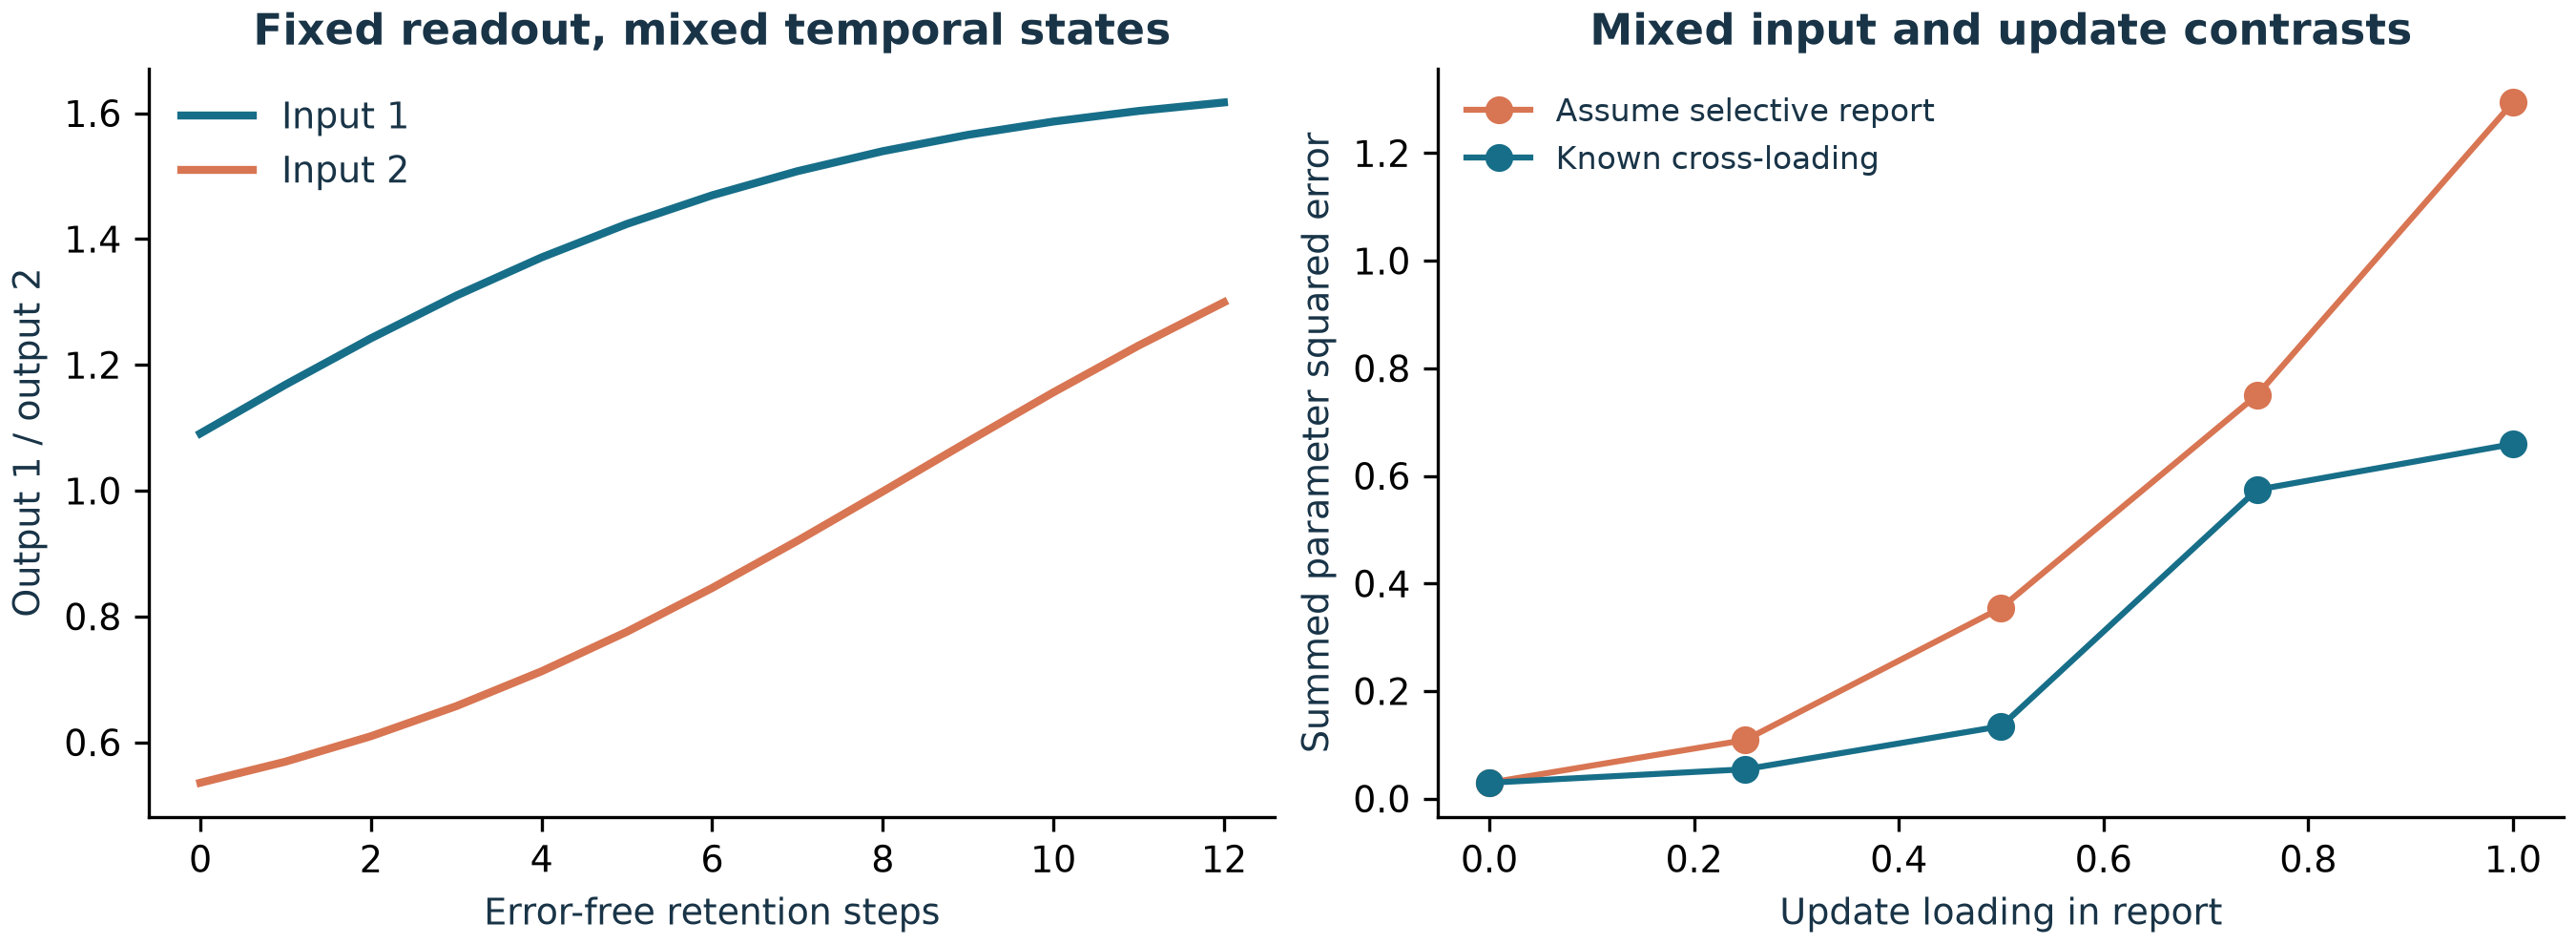
\includegraphics[width=\textwidth]{counterexamples.png}\end{center}
左：固定读出双模式的精确构造。右：已知或错误设为零的报告交叉载荷下，纯机制与混合因子的模拟参数误差。此处为构造反例及模拟误差，与人体测量分别报告。载荷为1的奇异情形保留因子分解歧义。
\clearpage\section{保留噪声结构的模型恢复}
每行包含20个新生成实例。列为拟合突然暴露后，在渐变暴露预测中强制选出的标签。参数扰动及噪声抽样为新增，生成家族及正则值来自视觉误差来源研究。来源残差保留通道配对及五块片段。该结果为特定方案诊断，具有有限蒙特卡洛精度。
\begin{center}\begin{tabular}{lrrrr}\toprule True / selected & C1 & S1 & C2 & S2\\\midrule
C1 & 7 & 6 & 5 & 2\\
S1 & 6 & 4 & 6 & 4\\
C2 & 0 & 0 & 15 & 5\\
S2 & 0 & 0 & 5 & 15\\
\bottomrule\end{tabular}\end{center}
\section{交叉载荷压力测试：纯机制及混合变化}
该测试使用设定的归一化报告噪声SD 0.05、因子范数0.8，每格500个实例。参数误差为四个输入及四个更新系数平方误差之和。已知载荷及错误零载荷模型均用精确最小二乘。载荷为1时已知模型的秩为1，最小范数解保留机制非唯一性。
\small\begin{longtable}{llrrr}\toprule Loading & Truth & Wrong-model error & Known-loading error & Rank\\\midrule\endhead
0.00 & input & 0.0306 & 0.0306 & 2\\
0.00 & update & 0.0296 & 0.0296 & 2\\
0.00 & mixture & 0.0296 & 0.0296 & 2\\
0.25 & input & 0.0311 & 0.0563 & 2\\
0.25 & update & 0.1122 & 0.0537 & 2\\
0.25 & mixture & 0.1090 & 0.0546 & 2\\
0.50 & input & 0.0291 & 0.1254 & 2\\
0.50 & update & 0.3512 & 0.1299 & 2\\
0.50 & mixture & 0.3546 & 0.1346 & 2\\
0.75 & input & 0.0311 & 0.5962 & 2\\
0.75 & update & 0.7476 & 0.6036 & 2\\
0.75 & mixture & 0.7501 & 0.5742 & 2\\
1.00 & input & 0.0308 & 0.3226 & 1\\
1.00 & update & 1.3141 & 0.3224 & 1\\
1.00 & mixture & 1.2941 & 0.6593 & 1\\
\bottomrule\end{longtable}\normalsize
\section{独立定位数据检查}
\textbf{30implicit (n=20)} 主动、被动、主动减被动变化：-6.43 [-8.62, -4.04], -4.89 [-6.93, -3.12], -1.54 [-2.91, -0.12]\par
\textbf{30explicit (n=21)} 主动、被动、主动减被动变化：-9.01 [-11.34, -6.61], -6.63 [-9.59, -4.13], -2.38 [-4.14, -0.34]\par
\textbf{cursorjump (n=20)} 主动、被动、主动减被动变化：-5.68 [-7.47, -3.84], -3.85 [-5.39, -2.35], -1.84 [-3.05, -0.52]\par
\textbf{handview (n=29)} 主动、被动、主动减被动变化：-3.24 [-5.78, -1.11], -3.22 [-6.04, -0.82], -0.02 [-0.86, 0.81]\par
区间采用参与者重采样，平均作者插值得到的三个空间方向。对照/指示组曾用于更早发表研究，此处只计数一次。该重分析检验单研究中的报告选择性，与跨研究力场预测分别报告。
\section{优化与数值表示}
64初值来源内审计用新随机种子与64初值最终拟合比较，最大损失改善为：1.13e-10. 接近极点采用差商表示，避免相反系数抵消。随附仅来源基线迁移评分、完整优化记录、数据哈希及来源提取核查。

\begingroup\fontsize{8.5}{9.6}\selectfont\setlength{\parskip}{0pt}\setlength{\bibsep}{1pt}\bibliographystyle{unsrtnat}\bibliography{references}\endgroup\end{document}